\section{Korištenje programske podrške}
Programska podrška napravljena u svrhu demonstracije svih spomenutih značajki ima dva glavna načina rada.
Ispis pronađenog teksta i pretraga unešenog teksta.
\subsection{Ispis pronađenog teksta}
Način rada koji se pretpostavlja da korisnik želi koristiti.
Kroz argument predaje se apsolutna putanja do slike nad kojom se želi izvršiti detekcija a program na standardni izlaz ispisuje pronađeni tekst.
Pronađeni tekst zatim prolazi evaluaciju koja je dio standardne biblioteke programskog jezika \emph{Python}.
Ako je izraz moguće evaluirati npr. "$2 + 2$", na standardni izlaz ispisuje se rezultat operacije kao što je vidljivo na slici ~\ref{fig:output}.
\begin{figure}[h!]
	\centering
	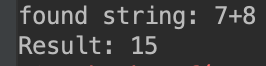
\includegraphics[width=0.6\linewidth]{CommandLineOutput}
	 \caption{Izlaz nakon evaluacije pronađenog teksta}
 	 \label{fig:output}
\end{figure}
\subsection{Pretraga unešenog teksta}
Drugi način rada nakon što slika prođe kroz korak detekcije i klasifikacije teksta sprema pronađeni izraz u obliku niza.
Korisnik pri izvršavanju programa prethodno mora unjeti regularni izraz koji opisuje ono što želi znati nalazi li se na slici na što program odgovara na standardni izlaz postoji li ili ne.
Način pretrage unešenog teksta dostupan je postavljanjem zastavice \texttt{r} kao argument pri pokretanju.
\section{Budući rad}
Iako programska podrška trenutno pruža osnovnu funkcionalnost, postoji dosta prostora za rast i napredak.
Trebala bi se znati vršiti segmentacija izraza po retcima jer se trenutno pronađeni objekti sortiraju s lijeva na desno i na isti način evaluiraju.
Segmentacija po retcima pružila bi mogućnost za kompliciranije izraze i kompletniju implementaciju. \\
Također, bilo bi korisno mrežu spojiti sa jednostavnim grafičkim sučeljem koje bi znatno olakšalo korištenje van komandne linije.
